\documentclass[tikz]{standalone}

\usepackage{amsmath}
\usepackage{circuitikz}

\usetikzlibrary{positioning}

\let\Re\undefined
\let\Im\undefined
\DeclareMathOperator{\Re}{\operatorname{Re}}
\DeclareMathOperator{\Im}{\operatorname{Im}}

\begin{document}
	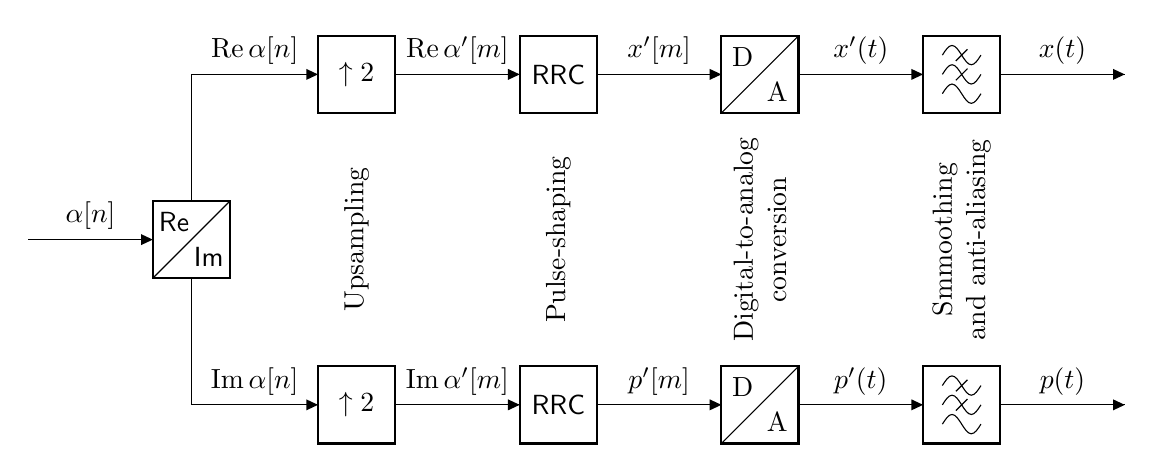
\begin{tikzpicture}[
		node distance=4.5em,
	]
		\coordinate (in) at (0,0);
		\node (cri) [twoportsplitshape, right=of in, circuitikz/t1=\textsf{Re}, circuitikz/t2=\textsf{Im}] {};
		\node (ups1) [twoportshape, above right=of cri, t=$\uparrow2$] {};
		\node (psh1) [twoportshape, right=of ups1, t=\textsf{RRC}] {};
		\node (dac1) [dacshape, right=of psh1] {};
		\node (lwp1) [lowpassshape, right=of dac1] {};
		\coordinate[right=of lwp1] (out1);
		\node (ups2) [twoportshape, below right=of cri, t=$\uparrow2$] {};
		\node (psh2) [twoportshape, right=of ups2, t=\textsf{RRC}] {};
		\node (dac2) [dacshape, right=of psh2] {};
		\node (lwp2) [lowpassshape, right=of dac2] {};
		\coordinate[right=of lwp2] (out2);
		
		\draw (in) -- (cri.west) node[above, midway, sloped]{$\alpha[n]$} node[inputarrow]{};

		\draw (cri.north) -- (cri.north|-ups1.west) -- (ups1.west) node[above, midway, sloped]{$\Re{\alpha[n]}$} node[inputarrow]{};
		\draw (ups1.east) -- (psh1.west) node[above, midway, sloped]{$\Re{\alpha^\prime[m]}$} node[inputarrow]{};
		\draw (psh1.east) -- (dac1.west) node[above, midway, sloped]{$x^\prime[m]$} node[inputarrow]{};
		\draw (dac1.east) -- (lwp1.west) node[above, midway, sloped]{$x^\prime(t)$} node[inputarrow]{};
		\draw (lwp1.east) -- (out1) node[above, midway, sloped]{$x(t)$} node[inputarrow]{};

		\draw (cri.south) -- (cri.south|-ups2.west) -- (ups2.west) node[above, midway, sloped]{$\Im{\alpha[n]}$} node[inputarrow]{};
		\draw (ups2.east) -- (psh2.west) node[above, midway, sloped]{$\Im{\alpha^\prime[m]}$} node[inputarrow]{};
		\draw (psh2.east) -- (dac2.west) node[above, midway, sloped]{$p^\prime[m]$} node[inputarrow]{};
		\draw (dac2.east) -- (lwp2.west) node[above, midway, sloped]{$p^\prime(t)$} node[inputarrow]{};
		\draw (lwp2.east) -- (out2) node[above, midway, sloped]{$p(t)$} node[inputarrow]{};
		
		\node at (ups1.north|-cri) [rotate=90] {Upsampling};
		\node at (psh1.north|-cri) [rotate=90] {Pulse-shaping};
		\node at (dac1.north|-cri) [text width=8em, align=center, rotate=90] {Digital-to-analog conversion};
		\node at (lwp1.north|-cri) [rotate=90, text width=8em, align=center] {Smmoothing and anti-aliasing};
	\end{tikzpicture}
\end{document}
